\documentclass[tikz,border=8pt]{standalone}
\usepackage{amsmath}\usepackage{pgfplots}\pgfplotsset{compat=1.18}
\definecolor{ink}{HTML}{21352F}\definecolor{teal}{HTML}{087F7B}\definecolor{gold}{HTML}{C58B2A}\definecolor{rose}{HTML}{B65A62}
\begin{document}
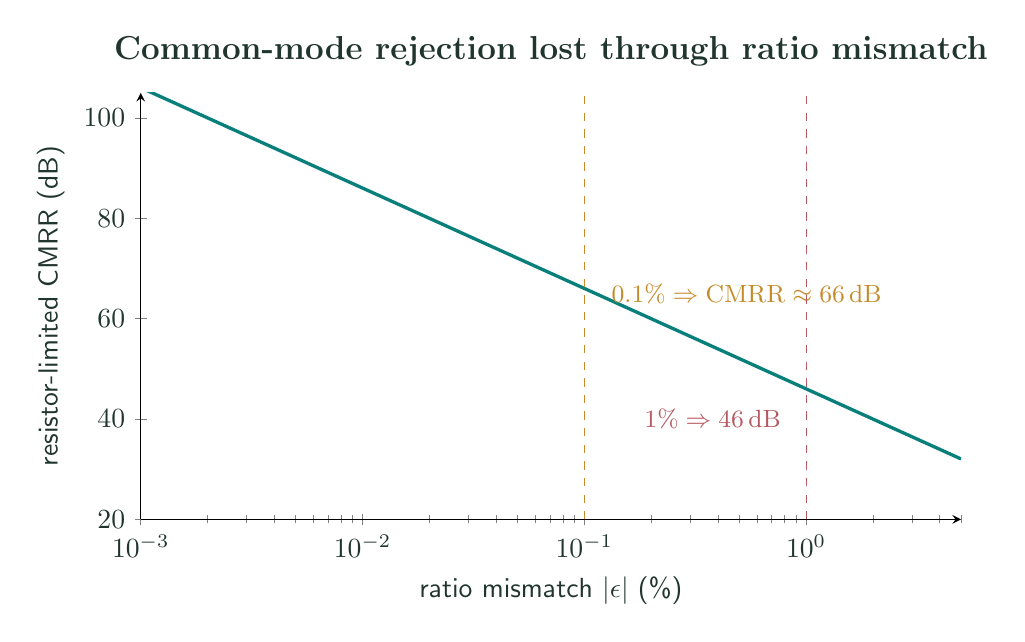
\begin{tikzpicture}[font=\sffamily,text=ink]
\begin{axis}[width=12cm,height=7cm,xmode=log,xmin=.001,xmax=5,ymin=20,ymax=105,axis lines=left,xlabel={ratio mismatch $|\epsilon|$ (\%)},ylabel={resistor-limited CMRR (dB)},title={Common-mode rejection lost through ratio mismatch},title style={font=\bfseries\large}]
 \addplot[teal,very thick,domain=.001:5,samples=260] {20*log10(200/x)};
 \draw[gold,dashed] (axis cs:.1,20)--(axis cs:.1,105);
 \node[gold,anchor=west,font=\small] at (axis cs:.12,65) {$0.1\%\Rightarrow \mathrm{CMRR}\approx66\,$dB};
 \draw[rose,dashed] (axis cs:1,20)--(axis cs:1,105);
 \node[rose,anchor=east,font=\small] at (axis cs:.85,40) {$1\%\Rightarrow46\,$dB};
\end{axis}
\end{tikzpicture}
\end{document}
